% Alexis Tercero: https://github.com/AlexisTercero55
%---------------------------------------------------------------------
%Plantilla para futuras entregas
\documentclass[12pt, letterpaper]{article}
\usepackage[utf8]{inputenc}
\usepackage[T1]{fontenc}
\usepackage[spanish,mexico]{babel}
% ajuste de margenes
\usepackage[left=2.5cm,right=2.5cm,top=2.5cm,bottom=2.5cm]{geometry}
\linespread{1}
\pagestyle{headings}
\setlength{\parindent}{0pt} % Elimina auto identacion en parrafos
%---------------------------------------------------------------------
%CONFIG DE TEOREMA
\usepackage{tikz,lipsum,lmodern}
\usepackage[most]{tcolorbox}
\newtcbtheorem[auto counter,number within=section]{theo}%
  {Theorem}{fonttitle=\bfseries\upshape, fontupper=\slshape,
     arc=0mm, colback=blue!5!white,colframe=blue!75!black}{theorem}
%---------------------------------------------------------------------
\usepackage{enumitem}% enumerates
\usepackage{verbatim} 
\usepackage{minted}%code listing
\usepackage{svg}
\usepackage{caption} %imgs dentro de enumerciones
\usepackage{amssymb}
\usepackage{amsmath}
\usepackage{tikz}
\usetikzlibrary{calc, arrows}
%\usepackage{xcolor} %{\color{blue} texto}
\usepackage{xcolor}%[dvipsnames]
\definecolor{mygreen}{RGB}{29, 131, 72}
\usepackage{mathtools}
\usepackage{epigraph}%epígrafe \epigraph{text}{\textit{Richard Courant}}
\usepackage{dirtytalk}%\say{}
\usepackage{graphicx}%imagenes en texto
\usepackage{hyperref}% para hipervinculos
\hypersetup{
    colorlinks=true,
    linkcolor=blue,
    filecolor= {35, 155, 86},      
    urlcolor=mygreen,
    pdftitle={Alexis Tercero},
    pdfpagemode=FullScreen,
    }
%---------------------------------------------------------------------
\author{Alexis Tercero: alexistercero55@gamil.com}
% elimina las ojas blancas extras despues del titulo y tabla de contenidos
\let\cleardoublepage=\clearpage 
%---------------------------------------------------------------------
%---------------------------------------------------------------------
%---------------------------------------------------------------------
\begin{document}
%---------------titulo-----------------------------------------------

%------------------------------------------------------------
%------------------------------------------------------------

\rule{\textwidth}{1pt}
\begin{center} %indicador de seccion/ introducion
    \bfseries Tarea 1 \\ Alexis Uriel Tercero López\\Uso de primitivas de dibujo en OpenGL
\end{center}
\rule{\textwidth}{1pt}

\begin{itemize}
    \item Sistema operativo: Windows 10
    \item Compilar con: gcc TAREA1.c -lfreeglut -lopengl32
\end{itemize}

\section{Código fuente}
\begin{minted}
[
frame=lines,
framesep=2mm,
baselinestretch=1.2,
fontsize=\scriptsize,
linenos %numeracion de lineas
]
{c}
/*  Alexis Tercero: https://github.com/AlexisTercero55
    build command: gcc TAREA1.c -lfreeglut -lopengl32
    build task@\.vscode\task.json : ctrl + shift + b

    Programa en lenguaje C/C++ que inicializará
    una ventana de GLUT/FreeGLUT donde se desplegarán dibujos 2D de 
    letras AUT: Alexis Uriel Tercero, cada una con un color diferente.

    Mientras se ejecuta el programa, el usuario podrá presionar teclas en su teclado,
    esperando ver una respuesta en el programa de acuerdo con:
        TECLA 1:    Las iniciales se dibujan con puntos
        TECLA 2:    Las iniciales se dibujan con líneas
        TECLA 3:    Las iniciales se dibujan con polígonos
        TECLA ESC:  Termina el programa
        TECLA OTRA: No pasa nada
*/
#include <stdlib.h>
#include <GL/glut.h>
#include <math.h>

/*PROTOTIPOS*/
//Plantilla
void configVentanaGlut(void);
void dibujar(void);
void teclado (unsigned char key, int x, int y);
//Tarea 1 : DIBUJAR INICIALES
void graficador2D(float (*f) (float),float a, float b, int n, int ord);
void tarea_lineas(void);
void tarea_puntos(void);
void tarea_poligonos(void);
float arco1_A(float x);
float arco2_A(float x);
float arco1_U(float x);
float arco2_U(float x);
void puntos_T(void);

int dibujar_con = 1;

int main(int argc, char** argv) 
{
    glutInit(&argc, argv);
    configVentanaGlut();
    //registro y ejecuccion de procesos
    glutDisplayFunc(dibujar);
    glutKeyboardFunc(teclado);

    glutMainLoop();

    return 0;
}

void configVentanaGlut(void)
{
    //configuracion de pantalla
    glutInitWindowSize(800, 600);
    glutInitWindowPosition(0,0);
    glutCreateWindow("Alexis Tercero 8/27/21 Tarea 1: DIBUJAR INICIALES");
}

void tarea_poligonos(void)
{
    /*INICIALES A U T CON POLIGONOS*/
    //A : verde
    glColor3f(0,1,0);
    glBegin(GL_POLYGON);//CCW
        graficador2D(arco2_A, -0.64, -0.42, 50, 1);
        graficador2D(arco1_A, -0.99, -0.28, 100, 0);
        graficador2D(arco2_A, -0.85, -0.64, 50, 1);
    glEnd();

    glBegin(GL_POLYGON);//CCW
        glVertex2f(-0.82, 0.2);//barra 2
        glVertex2f(-0.46, 0.2);
        glVertex2f(-0.48, 0.3);
        glVertex2f(-0.79, 0.3);//barra 1
    glEnd();

    //U : AMARILLA 
    glColor3f(1,1,0);
    glBegin(GL_POLYGON);//CCW
        graficador2D(arco1_U, 0, 0.44, 50, 1);
        graficador2D(arco2_U, -0.33, 0.33, 100, 0);
        graficador2D(arco1_U, -0.44, 0, 50, 1);
    glEnd();

    //T : ROJA uwu
    glColor3f(1,0,0);
    glBegin(GL_POLYGON);//CCW
        puntos_T();
    glEnd();
}

void tarea_lineas(void)
{
    /*INICIALES A U T CON LINEAS*/
    //A : verde
    glColor3f(0,1,0);
    glBegin(GL_LINE_LOOP);//CCW
        graficador2D(arco2_A, -0.85, -0.42, 100, 1);
        graficador2D(arco1_A, -0.99, -0.28, 100, 0);
    glEnd();

    glBegin(GL_LINE_LOOP);//CCW
        glVertex2f(-0.82, 0.2);//barra 2
        glVertex2f(-0.46, 0.2);
        glVertex2f(-0.48, 0.3);
        glVertex2f(-0.79, 0.3);//barra 1
    glEnd();

    //U : AMARILLA 
    glColor3f(1,1,0);
    glBegin(GL_LINE_LOOP);//CCW
        graficador2D(arco1_U, -0.44, 0.44, 100, 1);
        graficador2D(arco2_U, -0.33, 0.33, 100, 0);
    glEnd();

    //T : ROJO
    glColor3f(1,0,0);
    glBegin(GL_LINE_LOOP);//CCW
        puntos_T();
    glEnd();
}

void tarea_puntos(void)
{
    /*INICIALES A U T CON PUNTOS*/
    //A : verde
    glColor3f(0,1,0);
    glBegin(GL_POINTS);
        graficador2D(arco2_A, -0.85, -0.42, 100, 1);
        graficador2D(arco1_A, -0.99, -0.28, 100, 0);
        glVertex2f(-0.82, 0.2);//barra 2
        glVertex2f(-0.46, 0.2);
        glVertex2f(-0.48, 0.3);
        glVertex2f(-0.79, 0.3);//barra 1
    glEnd();

    //puntos extras solo para tarea_puntos
    glBegin(GL_POINTS);
        glVertex2f(-0.75, 0.3);
        glVertex2f(-0.7, 0.3);
        glVertex2f(-0.65, 0.3);
        glVertex2f(-0.6, 0.3);
        glVertex2f(-0.55, 0.3);
        glVertex2f(-0.51, 0.3);
        
        glVertex2f(-0.78, 0.2);
        glVertex2f(-0.75, 0.2);
        glVertex2f(-0.70, 0.2);
        glVertex2f(-0.65, 0.2);
        glVertex2f(-0.6, 0.2);
        glVertex2f(-0.55, 0.2);
        glVertex2f(-0.50, 0.2);
    glEnd();

    //U : AMARILLA 
    glColor3f(1,1,0);
    glBegin(GL_POINTS);
        graficador2D(arco1_U, -0.44, 0.44, 100, 1);
        graficador2D(arco2_U, -0.33, 0.33, 100, 0);
    glEnd();

    //T : BLANCO
    glColor3f(1,1,1);
    glBegin(GL_POINTS);
        puntos_T();
        //puntos extras
        glVertex2f(0.9, 0.4);
        glVertex2f(.99, 0.5);
        glVertex2f(0.9, 0.6);
        glVertex2f(0.8, 0.6);
        glVertex2f(0.7, 0.6);
        glVertex2f(0.6, 0.6);
        glVertex2f(0.5, 0.6);
        glVertex2f(0.4, 0.5);
        glVertex2f(0.5, 0.4);
        glVertex2f(0.6, 0.2);
        glVertex2f(0.7, 0);
        glVertex2f(0.8, 0.2);
    glEnd();
}

float arco1_A(float x)
{
    return -pow(2.5*x + 1.6, 2) + 0.8;//math.h
}

float arco2_A(float x)
{
    return -2*pow(2.5*x + 1.6, 2) + 0.6;//math.h
}

float arco1_U(float x)
{
    return pow(2*x,2);
}

float arco2_U(float x)
{
    return pow(2.5*x,2) + 0.1;
}

void puntos_T(void)
{   //CCW
    glVertex2f(0.8, 0.4);//F
    glVertex2f(0.99, 0.4);//G
    glVertex2f(0.99, 0.6);//H
    glVertex2f(0.4, 0.6);//A
    glVertex2f(0.4, 0.4);//B
    glVertex2f(0.6, 0.4);//C
    glVertex2f(0.6, 0);//D
    glVertex2f(0.8, 0);//E
}

void graficador2D(float (*f) (float), float a, float b, int n, int orden)
{
    float x,y, paso = (b-a)/n; 

    if(orden)
    {
        x = a;
        for(int i=0; i<n; ++i)
        {
            y = f(x);
            glVertex2f(x, y);
            x += paso;
        }
    } 
    else
    {
        x = b;
        for(int i=0; i<n; ++i)
        {
            y = f(x);
            glVertex2f(x, y);
            x -= paso;
        }
    }
        
}

void dibujar(void) 
{
    glClear(GL_COLOR_BUFFER_BIT | GL_DEPTH_BUFFER_BIT);
    switch (dibujar_con)
    {
        case 1:
            tarea_puntos();
            break;
        case 2:
            tarea_lineas();
            break;
        case 3:
            tarea_poligonos();
            break;
        default:
            break;
    }
    glFinish();//que se muestre ya
    //glutSwapBuffers();
}

void teclado (unsigned char key, int x, int y) 
{
    switch (key) 
    {
        case 27: //scape in ASCII
            exit(0);
            break;
        case '1':
            dibujar_con = 1;
            break;
        case '2':
            dibujar_con = 2;
            break;
        case '3':
            dibujar_con = 3;
            break;
        default:
            break;
    }
    //INDICAR AL OS QUE DIBUJE YA
    glutPostRedisplay(); //optimizacion de recursos
}
\end{minted}
%-------------------------------------------------------
\section{Salida del programa: capturas de pantalla}
\begin{figure}[h!]
    \centering
    \includegraphics[scale=0.6]{4.png}
\end{figure}
\newpage
\begin{figure}[h!]
    \centering
    \includegraphics[scale=0.6]{5.png}
\end{figure}
\begin{figure}[h!]
    \centering
    \includegraphics[scale=0.6]{6.png}
\end{figure}
\newpage
%-------------------------------------------------------
\section{Extras}

\subsection{Boceto del dibujo}
\begin{figure}[h!]
    \centering
   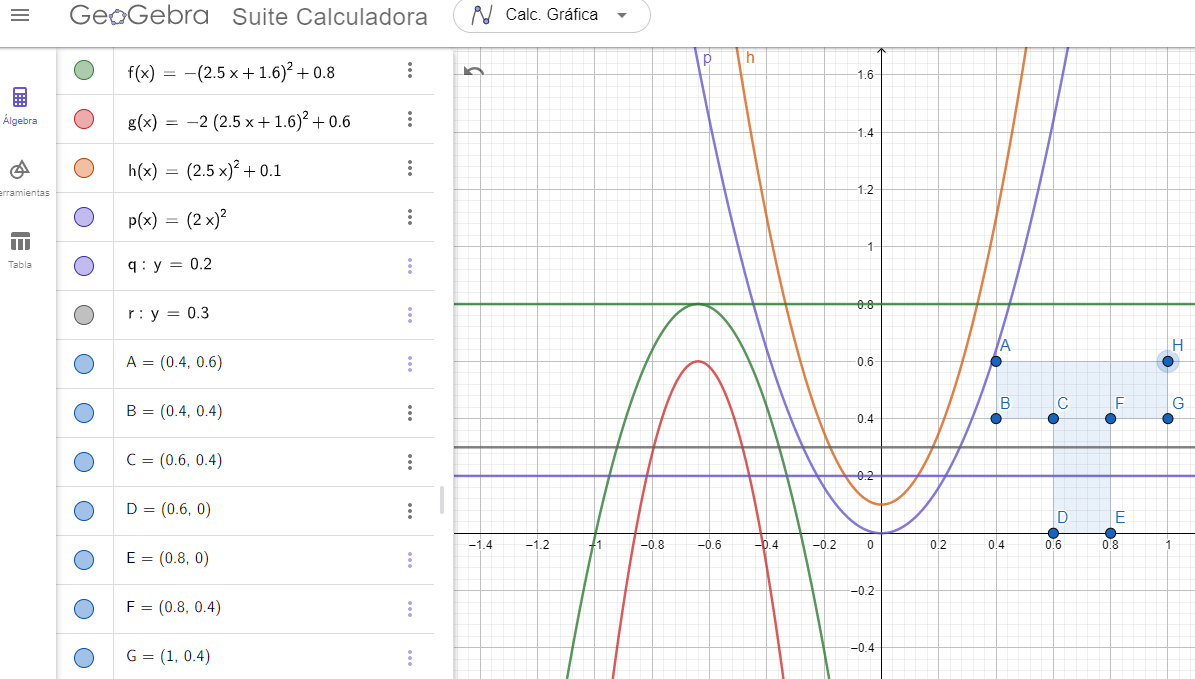
\includegraphics[scale=0.5]{help.png}
\end{figure}

\subsection{GitHub}
Se invita al lector a visitar el repositorio remoto 
\href{https://github.com/AlexisTercero55/practicasOpenGL}{AlexisTercero55/practicasOpenGL}
creado con el fin de registrar el aprendizaje a lo largo del curso. En el repositorio usted podrá encontrar notas del curso, practicas y tareas a través de la rama master.\vspace{2ex}

URL: \url{https://github.com/AlexisTercero55/practicasOpenGL}




%\hspace{1ex} \vspace{1ex} \begin{pmatrix}\end{pmatrix} \mathbb{R} \vrule ¿?\langle  \rangle \Big(\Big) \left|  \right|
%Wolfram command for jacobian jacobian matrix () with respect to (x_1,x_2,x_3)
\end{document}